\part{Spectroscopic estimation of the photon number for superconducting Kerr parametric oscillators
}\section{Introduction}
近年,Kerr非線形パラメトリック振動子(Kerr nonlinear parametric oscillators,  KPOs)が注目されている~\cite{goto2016bifurcation,goto2019quantum,goto2019demand,wang2019quantum,grimm2020stabilization,yamaji2022spectroscopic}.
KPOは2光子励起によって駆動されたKerr非線形共振器が基礎になっており~\cite{PhysRevA.44.4704,PhysRevA.48.2494},これは超伝導の共振器を利用することで実現されている~\cite{bourassa2012josephson,meaney2014quantum,leghtas2015confining}.
KPOは回路モデル型量子コンピュータのための量子ビットとして使われている~\cite{cochrane1999macroscopically,goto2016universal,puri2017engineering,puri2020bias}.
さらに近年,KPOに関する量子散逸相転移が見つかっており,これは量子計測に利用できることが示されている~\cite{bartolo2016exact,minganti2018spectral,dykman2018interaction,rota2019quantum}. 

KPOは回路型量子コンピュータだけでなく,量子アニーリングの実現する素子としても有力な候補であることが知られている~\cite{goto2016bifurcation,puri2017quantum}.
量子アニーリングは組合せ最適化問題を解くためのテクニックの一つである~\cite{kadowaki1998quantum,farhi2001quantum}.
解くべき問題の解をIsing Hamiltonianの基底状態に埋め込むことができ,断熱条件を満たしながらQAを実行した後,Ising Hamiltonianの基底状態(問題の解)を得ることができる.\cite{morita2008mathematical}. 

重要なのは,KPOのHamiltonianがIsing Hamiltonianへマップすることができるということである~\cite{goto2016bifurcation,puri2017quantum}.
初期状態として真空状態を始め,パラメトリックドライブ項を断熱的に徐々に増加していくことで,KPOを用いたQAを実装することができる.このとき,KPOのネットワークは分岐過程を経てHamiltonianの基底状態を探し出す.
KPOを用いたQAの実現可能なアーキテクチャとして,最近接相互作用を用いたものが提案されている~\cite{lechner2015quantum,puri2017quantum}.
また,KPOの量子アニーリングへの応用は多岐にわたる~\cite{nigg2017robust,onodera2020quantum,2020CmPhy...3..235G}.

しかし, Ising HamiltonianをKPO Hamiltonianに正確にマップするためには,各KPOそれぞれの平均光子数の精密な制御が必要となる.半古典近似により,KPOの平均光子数を計算する公式はあるが,公式による計算値は実際の値と異なることがある~\cite{kanao2021high}.
そのため,実用的な組合せ最適化問題を解くためには,KPOの平均光子数の推定を確実に実行する手法が求められる.

\begin{figure}%[h]
\centering
		%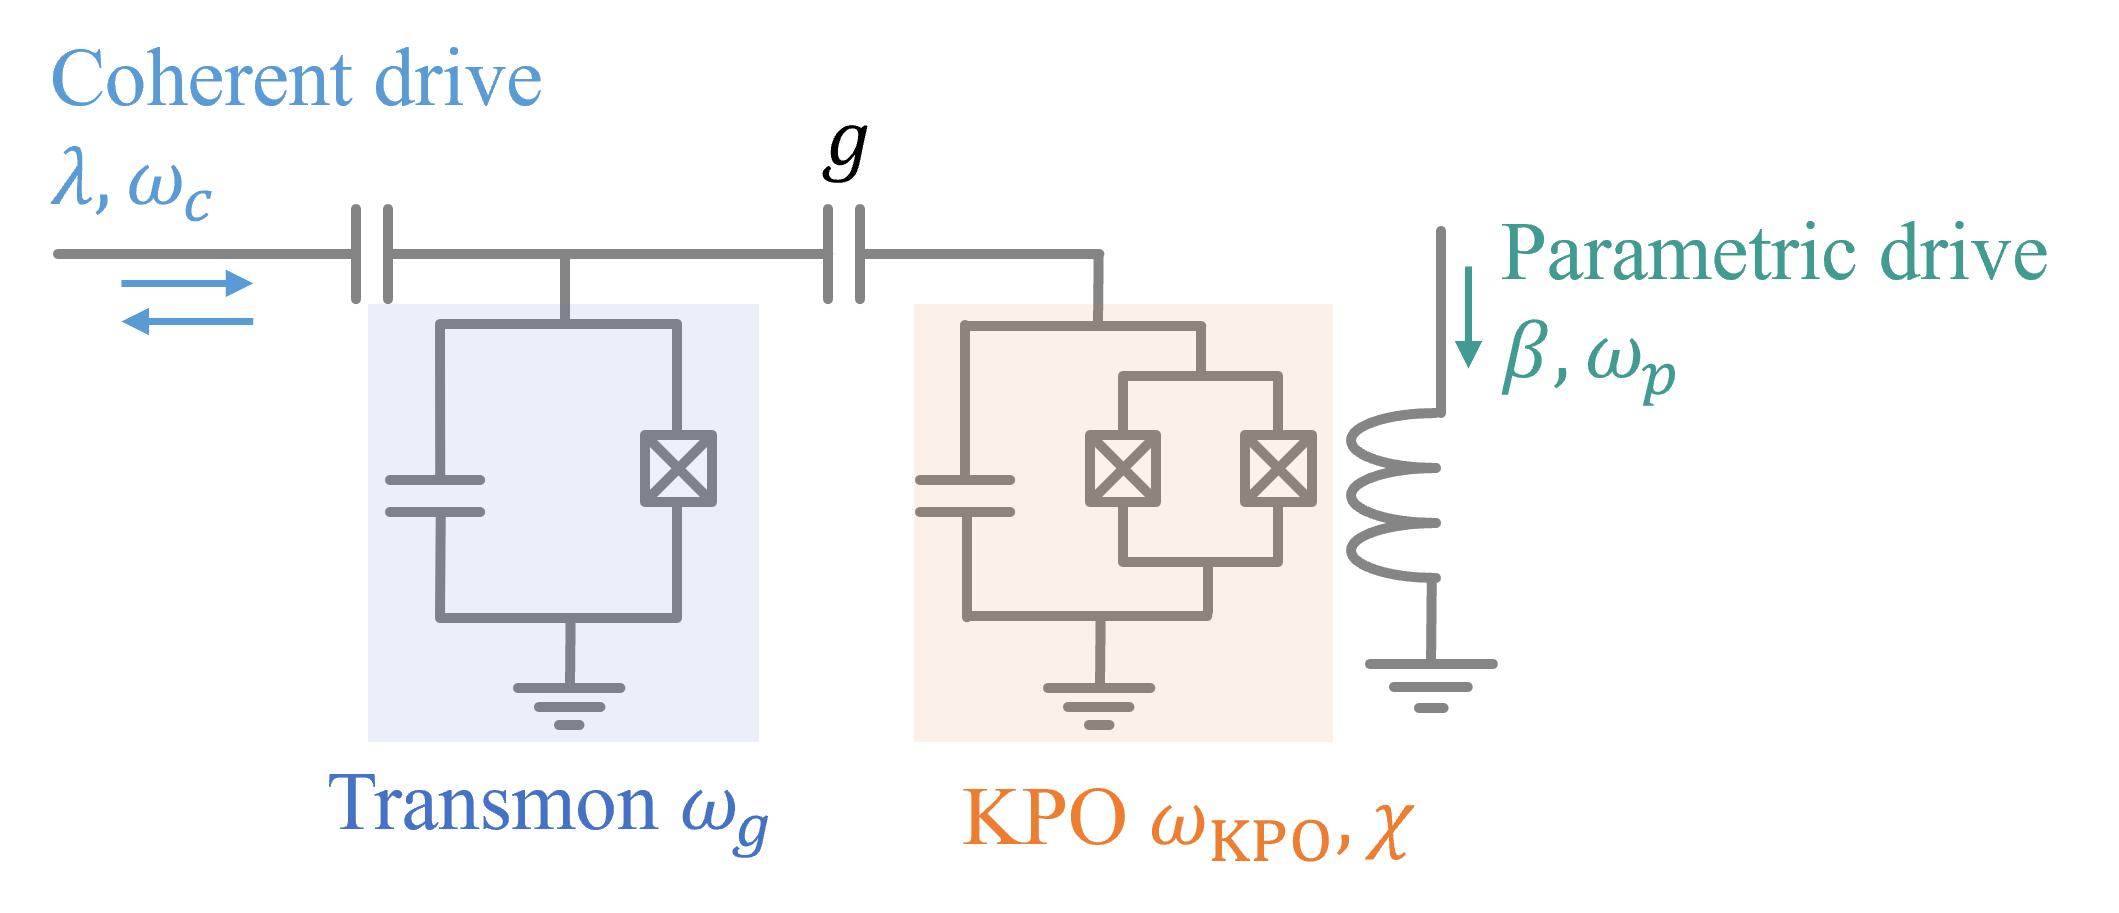
\includegraphics[width=9.1cm]{fig/fig1mod.png} \\
\caption{Schematic of a KPO coupled with a transmon qubit.
The transmon qubit is coupled to a transmission line. By driving the qubit through the transmission line and measuring the reflected fields, we can readout the information of the transmon qubit.
%To measure the population of the transmon qubit, we couple a resonator with the transmon qubit.
}
\label{fig:schematic1}
\end{figure}

In this paper, we propose a method to estimate the number of photons of the KPO from spectroscopic measurement. We consider a system, where the KPO is coupled with an ancillary qubit such as a superconducting transmon qubit or another KPO (without parametric drive), as shown in Fig.~\ref{fig:schematic1}. 

\subsection{ポピュレーションの測定および読み出し方法について}
平均光子数を推定するためには,スペクトルを実験的に測定する必要がある.そのためには,量子ビットの$\hat{\sigma}_z$の値を測定する必要がある.だから,量子ビットの状態読み出しのための共振器が必要となる.しかし,我々の手法では,補助量子ビットとトランスミッションラインは結合しており,トランスミッションラインを通して,量子ビットを駆動し,反射場を測定することによって,量子ビットの情報(スペクトル)を読み出すことが可能である~\cite{astafiev2010resonance,masuda2021theoretical}.そのため,読み出し用の共振器は不要である.そのため,我々はスペクトルを測定するために,基本的に反射測定を利用し,分散読み出しはオプションとして使うことが可能である.分散読み出しを使用する場合は,トランズモン量子ビットのポピュレーションを測定するために,分散読み出し用 (dispersive readout) の量子ビットと共振器を結合させることも可能である~\cite{mallet2009single,walter2017rapid,vijay2011observation}.
We show that spectroscopic measurements on the ancillary qubit provide an estimate of the number of photons of the KPO. We evaluate the performance of our method with numerical simulations by solving a master equation and show that the proposed method is more accurate than the conventional method.
It is worth mentioning that, in our previous study, by numerical methods, we investigate a case only when the driving strength is weak and the rotating wave approximation is valid\cite{2022ssdmkm}.
On the other hand, in this paper, by using both numerical and analytical methods, we analyze the case with strong driving
where the rotating wave approximation is violated. 
Moreover, in this paper, we study how the performance of our scheme changes with the detuning of the KPO.
These results in this paper provide a deep understanding of our scheme to estimate the number of photons.

The paper is organized as follows. In Sec. II, we introduce a model of a KPO coupled with an ancillary qubit. In Sec. III, we describe our method to estimate the number of the photons of the KPO by spectroscopic measurements.
In Sec. IV, we evaluate the performance of our method by using numerical simulations.
In Sec. V, we conclude our discussion.
Throughout this paper, we set $\hbar=1$.






\section{MODEL HAMILTONIAN}\label{Model}
In this section, we introduce a model of a KPO coupled 
with an ancillary qubit.
The Hamiltonian is given by
\begin{align}
    \hat{H}&=\omega_{\rm{KPO}}\ \hat{a}^\dagger\hat{a} - \frac{\chi}{12} (\hat{a}+\hat{a}^\dagger)^4 + 2\beta (\hat{a} + \hat{a}^{\dagger})^2\cos{\omega_{\rm{p}} t}\nn[10pt]
    &+\frac{\omega_{\rm{g}}}{2}\hat{\sigma}_z
    +g(\hat{a}+\hat{a}^\dagger)\hat{\sigma}_x
    +\lambda \hat{\sigma}_x \cos{\omega_c t},
\end{align}
where $\hat{a}^\dagger$ ($\hat{a}$) is a creation
(annihilation) operator of the KPO, $\omega_{\rm{KPO}}$ is the frequency of the KPO, $\chi$ is the Kerr coefficient, $\beta$ is the amplitude of a parametric drive, $\omega_{\rm{p}}$ is the frequency of the
parametric drive, $\omega_{\rm{g}}$ is the frequency of the ancillary qubit, $g$ is the coupling 
strength between the
KPO and the ancillary qubit, 
and $\lambda$ $(\omega_c)$ is the amplitude (frequency) of the driving field for the qubit, respectively. Here, $\hat{\sigma}_x$ and $\hat{\sigma}_z$ denote the Pauli operators.
Moving into a rotating frame at the frequency of $\omega_{\rm{p}}/2$ and adapting the rotating wave approximation, the Hamiltonian is written as
\begin{align}\label{total hamiltonian}
  \hat{H}&=\hat{H}_{\rm{KPO}}+\hat{H}_{\rm{G}}+\hat{H}_{\rm{I}}+\hat{H}_{\rm{D}},\\[10pt]
    \hat{H}_{\rm{KPO}}&=\Delta \hat{a}^\dagger\hat{a} - \frac{\chi}{2} \hat{a}^\dagger\hat{a}^\dagger\hat{a}\hat{a} + \beta (\hat{a}^2 + \hat{a}^{\dagger 2})\\[10pt]
    \hat{H}_{\rm{G}}&=\frac{\omega_{\rm{g}}-\omega_{\rm{p}}/2}{2}\hat{\sigma}_z\\[10pt]
    \hat{H}_{\rm{I}}&=g(\hat{a}\hat{\sigma}_{+}+\hat{a}^\dagger\hat{\sigma}_{-})\\[10pt]
    \hat{H}_{\rm{D}}&=\lambda_{\rm{p}}\left(\hat{\sigma}_+ e^{-i(\omega_c-\omega_{\rm{p}}/2)t}+\hat{\sigma}_- e^{i(\omega_c-\omega_{\rm{p}}/2)t}\right),
\end{align}
where $\Delta = \omega_{\rm{KPO}} -\chi - \omega_{\rm{p}}/2$ denotes the detuning of the KPO,  $\lambda_{\rm{p}}={\lambda}/{2}$ denotes the Rabi frequency of the ancillary qubit, and $\hat{\sigma}_{\pm}$ denotes the ladder operator.
Throughout our paper, we set $\Delta <0$.
%, which is typical for the experiment~\cite{yamaji2022spectroscopic}.
The ground and the first excited states of $\hat{H}_{\rm{G}}$ are $|{\rm{g}}\rangle $ and $|{\rm{e}}\rangle $, respectively. With $\beta =0$, %the lowest for eigenstates  are (in ascending order) 
the Fock states
$\ket{n}$ (for $n=0,1,2, 3$) become eigenstates of the
$H_{\rm{KPO}}$. For $\beta \gg |\chi|$, on the other hand, the corresponding eigenstates are approximately given by $(|\alpha \rangle+ |-\alpha \rangle )/\sqrt{2}$, $(|\alpha \rangle- |-\alpha \rangle )/\sqrt{2}$, $({\it{D}}_{\alpha}+{\it{D}}_{-\alpha})|1\rangle /\sqrt{2}$, and 
$({\it{D}}_{\alpha}-{\it{D}}_{-\alpha})|1\rangle /\sqrt{2}$, where ${\it{D}}_{ \alpha}=\exp{(\alpha\hat{a}-\alpha^{\ast}\hat{a}^\dagger)}$
denotes a displacement operator~\cite{goto2016bifurcation}.



\subsection{分散読み出しによる平均光子数推定の困難さ}
トランズモン量子ビットが線形共振器(調和振動子)を結合してるとき,$H'_{\rm{I}}=g \hat{\sigma}_z \hat{a}^{\dagger} \hat{a}$で記述される分散的相互作用 (dispersive interaction) を実現することができる.
この場合,トランズモン量子ビットを用いることで,共振器の平均光子数を測定することができる~\cite{johnson2010quantum,PhysRevApplied.14.044022,PhysRevX.11.031045,PhysRevA.103.023705}. 
しかし,我々の知る限り,トランズモン量子ビットとパラメトリックドライブで駆動されるKPOとの間の分散的相互作用を実現する手法は存在しない.さらに,$H'_{\rm{I}}=g \hat{\sigma}_z \hat{a}^{\dagger} \hat{a}$ は$\hat{H}_{\rm{KPO}}$と非可換である.このような非可換な相互作用は測定対象系の情報を読み出すために適していないことが知られている \cite{endo2020projecting}.
原理的には,パラメトリックポンプと非線形性を素早くオフにすれば($\beta=\chi=0$),KPOは線形共振器と同等になり,KPOの周波数をトランスモン量子ビットの周波数から離調させることで分散的相互作用を実現することが可能である. 
しかし,この場合,パルス操作を含む高速な測定が必要となり,連続波の測定だけで済む我々の提案する手法よりもはるかに困難である.


回転座標系でのHamiltonianの導出については,Appendix\ref{}を参照


\section{Methods}
In this section, we propose a method to estimate the number of photons of the KPO from a spectroscopic measurement of an ancillary qubit coupled with the KPO. As we explained,
for sufficiently large $\beta$, the ground state of the KPO is approximately described by a superposition of two coherent states, namely $|\alpha\rangle$ and $|-\alpha\rangle$ where $\pm \alpha$ is the amplitude of the coherent state. Without loss of generality, we can assume that $\alpha$ is a real number. Then, the Hamiltonian of the ancillary qubit is approximately written as

\begin{align}\label{qubit_Hamiltonian}
    \hat{H}_{\rm{qubit}}^{\rm{eff}}
    &=\frac{\omega_{\rm{g}}-\omega_{\rm{p}}/2}{2}\hat{\sigma}_z
    \pm 
    g\alpha\ \hat{\sigma}_x\nn[10pt]
    &+\lambda_{\rm{p}}\left(\hat{\sigma}_+ e^{-i\Delta _{\rm{q}}t}+\hat{\sigma}_- e^{i\Delta _{\rm{q}}t}\right),
\end{align}
where $\Delta _{\rm{q}}=\omega_c-\omega_{\rm{p}}/2$ denotes a detuning of the coherent drive
%the ancillary qubit 
\cite{goto2016bifurcation}.


It is known that we can observe a Mollow triplet via a spectroscopic measurement with this Hamiltonian, where resonant transition frequencies are 
$\Delta _{\rm{q}}=0$, $\pm 2g\alpha$~\cite{Mollow:1969zz,wu1994phase,wrigge2008efficient,ulhaq2012cascaded,xu2007coherent,laucht2017dressed}.
Since we can estimate the value of $g$ from a separate spectroscopic measurement by observing a vacuum Rabi splitting \cite{wallraff2004strong,chiorescu2004coherent}, 
we can obtain the value of $\alpha$ from the peak (dip) positions observed in the Mollow triplet.
It is worth mentioning that our method using the ancillary qubit
may affect the dynamics of the KPO due to the resonant condition between the KPO and the ancillary qubit. This means that 
we may be unable to use our method to estimate the number of photons in the middle of computation. 


\subsection{量子計算中の本手法の影響について}
ただし,補助量子ビットを用いる本手法は,KPOと補助量子ビットが共振するため,KPOのダイナミクスに影響を与える可能性がある.
つまり,量子計算の途中で我々の手法を用いて光子数を推定することができなくなる可能性がある.  
しかし,量子アニーリングやゲート型量子計算では,計算終了時の読み出し直前で本手法を適用することができる.
また,計算を開始する前に本手法を用いて平均光子数を知ることも可能である.
このような場合,計算中に,KPOと補助量子ビットの間のdetuningを設定し,補助量子ビットがKPOのダイナミクスに影響を与えないようにすることができる.ただし,実際に解いているKPOのdetuningは変えないように注意する(計算中はトランズモンの共振周波数をKPOの共振周波数から離しておく).
したがって,本手法は,量子アニーリングやゲート型量子計算において特に有効であることがわかる.

QA前に本手法を用いて,KPOからの出力の振幅$|\alpha|^2$に対して光子数を求めておき,較正 (calibration) しておくことで,KPOからの出力の振幅を読むだけで光子数がわかる.


With a conventional method \cite{puri2017engineering}, an analytical formula under semi-classical approximations such as $\alpha_{\mathrm{ana}}=\sqrt{(2\beta+\Delta)/\chi}$ is used to estimate the number of photons of the KPO when $\beta$ is much larger than the decay rate $\gamma_1$.
% \YMdel{Strictly speaking, a decay rate $\gamma_1$ also affects the number of photons. However, since we use parameters $\beta$ which is much larger than the decay rate, we can ignore the effect of $\gamma_1$ for the estimation of the number of photons} %\cite{puri2017engineering}.
% \footnote{Strictly speaking, a decay rate $\gamma_1$ also affects the number of photons. However, since we use parameters $\beta$ which is much larger than the decay rate, we can ignore the effect of $\gamma_1$ for the estimation of the number of photons \cite{puri2017engineering}}. 
Importantly,
previous research shows that 
the
value 
of $\alpha_{\mathrm{ana}}=\sqrt{(2\beta+\Delta)/\chi}$
can provide a wrong estimate~\cite{kanao2021high} due to the violation of the approximation.
Therefore, it is crucial to adopt more reliable method to estimate the number of photons especially when the conventional method provides an inaccurate estimation.


\subsection{本手法を適用するための結合強度$g$について}
SSDMで質問があった,この手法が適応できる結合強度gについては,重要な点であると思うので,ぜひご検討いただけると幸いです.
単純にgと損失レートκとの比というよりは,コヒーレント状態の振幅αとの積,α*g(ピーク間の距離)と,おそらくκから決まるMollow triplet のピークの線幅の大きさの比で説明できるのでは?と期待しているのですが,いかがでしょうか?
もし,g=5MHz以外の計算,例えばgがκと同じくらい小さい時などの結果もあればぜひ見てみたいです.
私は既存のデバイスで実験したので,gは5MHzで固定でしたが,
この手法を利用することを想定して,新たにデバイスを設計しようと思った場合には,どういうgにする必要があるのかという示唆があると非常に有益であると思います


\section{Numerical simulations}
In this section, we evaluate the performance of our method by comparing with the conventional method using numerical simulations of the GKSL (Gorini-Kossakowski-Sudarshan-Lindblad) master equation.
Here, we adopt the Hamiltonian in Eq.~\eqref{total hamiltonian}.
To take the effect of photon loss into account, we use the following GKSL master equation

\begin{align}\label{Eq.GKSL}
\frac{\partial\rho}{\partial t} &= -i\left[\hat{H}_{\rm{KPO}}+\hat{H}_{\rm{G}}+\hat{H}_{\rm{I}}+\hat{H}_{\rm{D}} 
,\ \rho\right] \nn[10pt]
&+\frac{\gamma_1}{2} \left (2\hat a \rho \hat a^\dagger - \left\{ \hat a^\dagger \hat a, \rho \right\}\right)
+ \frac{\gamma_2}{2} \left (2\hat{\sigma}_{-} \rho \hat{\sigma}_{+} - \left\{ \hat{\sigma}_{+} \hat{\sigma}_{-}, \rho \right\}\right),
\end{align}
where $\gamma_1$ denotes the one photon dissipation rate of the KPO, $\gamma_2$ denotes the spontaneous emission rate of the ancillary qubit, and
$\hat{\rho}$ denotes the density matrix describing the quantum state of the total system.
We solve the GKSL master equation Eq.~\eqref{Eq.GKSL} using QuTiP~\cite{johansson2012qutip}.
We choose the initial state as a
steady state of Eq.~\eqref{Eq.GKSL} with $\lambda _{\rm{p}}=0$.
Also, we set $\omega_g=\omega_{\rm{p}}/2$.

\begin{figure}%[h]
\centering
		%\includegraphics[width=9.1cm]{fig/sigmaz_td_Detu_-30_Keer_18_pump_42_dec_0.8_L_0.5.pdf} \\
\caption{
(a) The time-integrated spectra $I$ against $\Delta_{\rm{q}}/2\pi$ with $\lambda_{\rm{p}}/2\pi=0.5$  MHz. We set the parameters as $\Delta/2\pi=-30.0$  MHz, $\chi/2\pi=18.0$ MHz, $\beta/2\pi=42.0$ MHz, $g/2\pi=5.0$ MHz, $\gamma_1/2\pi=\gamma_2/2\pi=0.8$ MHz, and $\omega_g=\omega_{\rm{p}}/2$.
(b)The energy diagram of the states of a KPO coupled with a qubit.
In the left (right) side, we show the energy diagram with $\beta/2\pi=0$ MHz ($\beta\gg |\chi|$). Here,
$|\alpha \rangle $ and $\ket{n}$ (for $n=0,1,2$) denote a coherent state
 and Fock states, respectively, while
${\it{D}}_{ \alpha}=\exp{(\alpha\hat{a}-\alpha^{\ast}\hat{a}^\dagger)}$
denotes the discplacement operator. 
% Here,
% $\ket{\rm{vac}}$,  $|\alpha \rangle $, and $\ket{n}$ (for $n=1,2$) denote the vacumme state, coherent state, and Fock states, respectively, while 
% %${\it{D}}_{\pm \alpha}$
% ${\it{D}}_{ \alpha}=\exp{(\alpha\hat{a}-\alpha^{\ast}\hat{a}^\dagger)}$
% denotes the discplacement operator. 
%such as ${\it{D}}_{\pm \alpha} |\rm{vac}\rangle = |\pm \alpha \rangle $. 
Also, $|g\rangle $ ($|e\rangle $) and $|\pm \rangle =\frac{1}{\sqrt{2}}(|g\rangle \pm |e\rangle )$
denotes the ground (excited) state and the superposition states of the qubit.
}
\label{fig:spect1}
\end{figure}




In Fig.~\ref{fig:spect1} (a), we plot a time-integrated spectra $I=(1/t)\int_{0}^{t}\ d\tau\ (\braket{\hat{\sigma}_z}+1)/2$ as a function of $\Delta_{\rm{q}}$ with a step of $0.05$ MHz,
where $\braket{\hat{\sigma}_z}={\rm{Tr}}[\hat{\sigma}_z \rho ]$,
which is effectively the same as a spectroscopy to detect the change in the pupulation of the qubit.

%\YM{We can interprete the three relevant transitions between them as the Mollow triplet of the ancillary qubit where the coupling with the KPO plays a role of the driving field on the qubit.}
%In Fig.~\ref{fig:spect1} (a),
This spectra is upper (lower) bounded by $1$ ($0$).
The value of this spectra depends on the Rabi frequency and decay rate of the qubit.
The observed peak and dips are at $\Delta_{\rm{q}}^{(0)}/2\pi=1.35$ MHz, $\Delta_{\rm{q}}^{(1)}/2\pi= -16.80$ MHz and $\Delta_{\rm{q}}^{(2)}/2\pi = 17.10$ MHz, respectively.
% The observed peaks are at $\Delta_{\rm{q}}^{(0)}/2\pi=1.35$ MHz, $\Delta_{\rm{q}}^{(1)}/2\pi= -16.80$ MHz , and $\Delta_{\rm{q}}^{(2)}/2\pi = 17.10$ MHz.

Fig.~\ref{fig:spect1} (b) shows the energy diagram composed of the system of the KPO coupled with an ancillary qubit.
We calculate the energy eigenvalues of the Hamiltonian, and we confirm that the energy difference between the eigenvalues is almost the same as the peak frequency observed in our numerical simulation.
The dip at $\Delta_{\rm{q}}^{(1)}/2\pi= -16.80$ MHz ($\Delta_{\rm{q}}^{(2)}/2\pi = 17.10$ MHz) corresponds to the transition between the ground (first excited) state and the second (third) excited state, which we describe by a red vertical arrow in Fig.~\ref{fig:spect1} (b).
Here, with our parameters, the ground state, first excited state, second excited state, and third excited state 
 are approximately described as
$\ket{-}(\ket{\alpha}+\ket{-\alpha})$,
$\ket{-}(\ket{\alpha}-\ket{-\alpha})$,
$\ket{+}(\ket{\alpha}+\ket{-\alpha})$, and
$\ket{+}(\ket{\alpha}-\ket{-\alpha})$, respectively.
%$\ket{-}(\hat{D}_{\alpha}+\hat{D}_{-\alpha})\ket{2}$ to $\ket{-}(\hat{D}_{\alpha}-\hat{D}_{-\alpha})\ket{2}$,  
 %$\ket{-}(\ket{\alpha}-\ket{-\alpha})$
 On the other hand, the peak at $\Delta_{\rm{q}}^{(0)}/2\pi=1.35$ MHz corresponds to a transition between the fourth excited state and the fifth excited state, which we describe by a green vertical arrow in Fig.~\ref{fig:spect1} (b),
 where the fourth (fifth) excited state is approximately given as $\ket{-}(\hat{D}_{\alpha}+\hat{D}_{-\alpha})\ket{2}$ ($\ket{-}(\hat{D}_{\alpha}-\hat{D}_{-\alpha})\ket{2}$).
Actually, from the numerical simulation, the population of the fourth  (fifth) excited state at $t=0$ is $0.00590$ (0.0173) and becomes finally $0.00772$ (0.0155) at $t=3$ $\mu$s. This means that the coherent drive actually induces a transition between the fourth excited state and the fifth excited state.
By diagonalizing the Hamiltonian, we recognized that we have a transition between the second excited state and the third excited state
 with an energy difference of
 $2\pi \times 0.5$ MHz.
 However, we cannot resolve this peak in the numerical simulation possibly due to the large width of the peak at $\Delta_{\rm{q}}^{(0)}$.




% \KM{In Fig.~\ref{fig:pump_effect}, we describe a effect of an parametric drive occur the transition $\Delta E_{4,5}$.
% In Fig.~\ref{fig:pump_effect}, we plot a transition frequency $\Delta_{\rm{q}}^{(0)}$ against a amplitude of a parametric drive $\beta$.
% From Fig.~\ref{fig:pump_effect}, we find $\Delta_{\rm{q}}^{(0)}$ is equal to $\Delta E_{4,5}$ at $\beta/2\pi/ = 42.0$ MHz.}

Now, let us discuss the estimation of the number of photons.
We consider a steady state $\hat{\rho}_{\rm{ss}}$ of Eq.~\eqref{Eq.GKSL} with $\lambda_{\rm{p}}=0$ and $g=0$, and we define $\rm{Tr}[\rho_{\rm{ss}}\hat{a}^\dagger\hat{a}]=|\alpha|^2$.
Let us define a
 relative error of $|\alpha|^2$ estimated by using our method as $\epsilon_1\equiv||\alpha_{\rm{est}}|^2-|\alpha|^2|/|\alpha|^2$, where $|\alpha|^2$($|\alpha_{\rm{est}}|^2$) is the actual (estimated) value of the photon number of the KPO.
Also, when we use the analytical formula, the relative error of the estimated $|\alpha|^2$ is
defined as $\epsilon_2\equiv||\alpha_{\rm{ana}}|^2-|\alpha|^2|/|\alpha|^2$.

From Fig.~\ref{fig:spect1} (a), we observe two dips at
$\Delta ^{(1)}_{\rm{q}}$ and $\Delta ^{(2)}_{\rm{q}}$ and the frequency difference is $(\Delta ^{(2)}_{\rm{q}}-\Delta ^{(1)}_{\rm{q}})/2\pi=33.90$ MHz. We can estimate the number of photons from this, as we explained before.
Since we set $g/2\pi=5$ MHz, 
we obtain an estimated value of 
$|\alpha _{\rm{est}}|^2= 2.87$,
where we solve an equation of $4g\alpha _{\rm{est}}/2\pi=(\Delta ^{(2)}_{\rm{q}}-\Delta ^{(1)}_{\rm{q}})/2\pi=33.90$ MHz.
The relative error is calculated as
$\epsilon_1=0.0280$.
On the other hand, when we use the analytical formula, we obtain $\epsilon_2=0.0672$.
This result indicates that our method provides a more accurate estimate of $\alpha$ than the conventional method. 

% \KM{Here, we observe the peak at $1.3$ MHz which shifted from $0$ MHz.
% We consider this shift is caused by a effect of the pump.
% We plot plot }

\begin{figure}%[h]
\centering
		%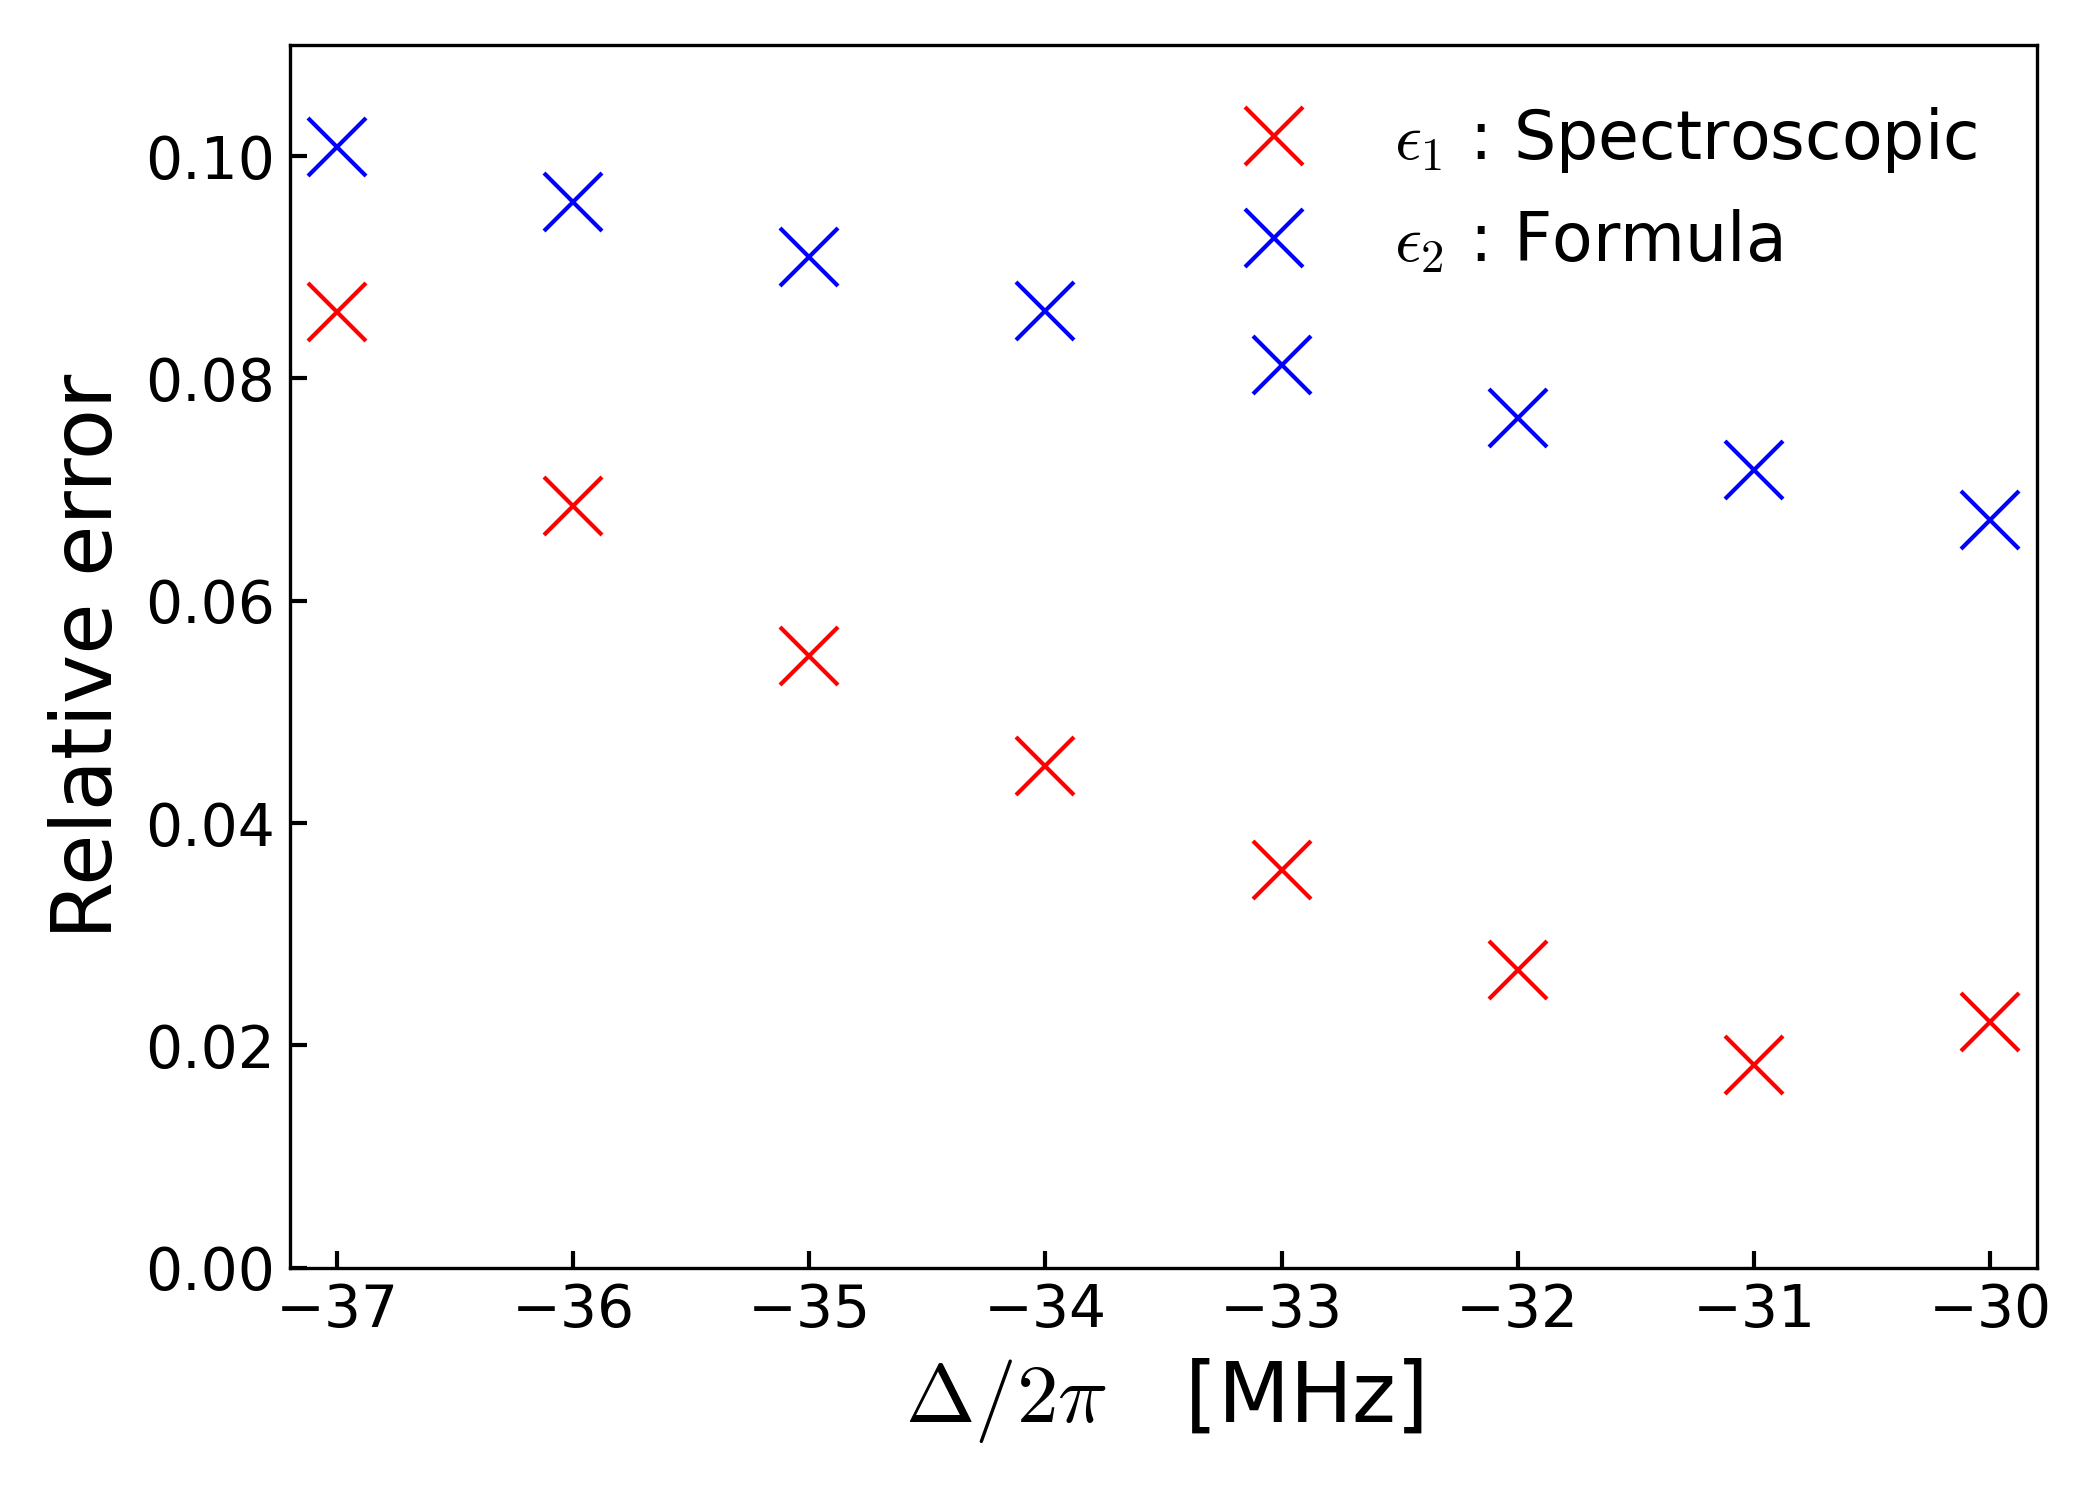
\includegraphics[width=9.1cm]{fig/alpha_estimete_meannum.png} \\
\caption{
Plot of the relative error $||\alpha_{\rm{est}}|^2-|\alpha|^2|/|\alpha|^2$ 
against the detuning of the KPO
 where $|\alpha|^2$ ($|\alpha_{\rm{est}}|^2$) is the true (estimated) value of the photon number.
 We set the parameters as $\chi/2\pi=18.0$ MHz, $\beta/2\pi=42.0$ MHz, $g/2\pi=5.0$ MHz, $\lambda_{\rm{p}}/2\pi=0.5$ MHz, $\gamma_1/2\pi=\gamma_2/2\pi=0.8$ MHz, and $\omega_g=\omega_{\rm{p}}/2$.
}
\label{fig:spec_error1}
\end{figure}

 

\begin{figure}%[h]
\centering
		%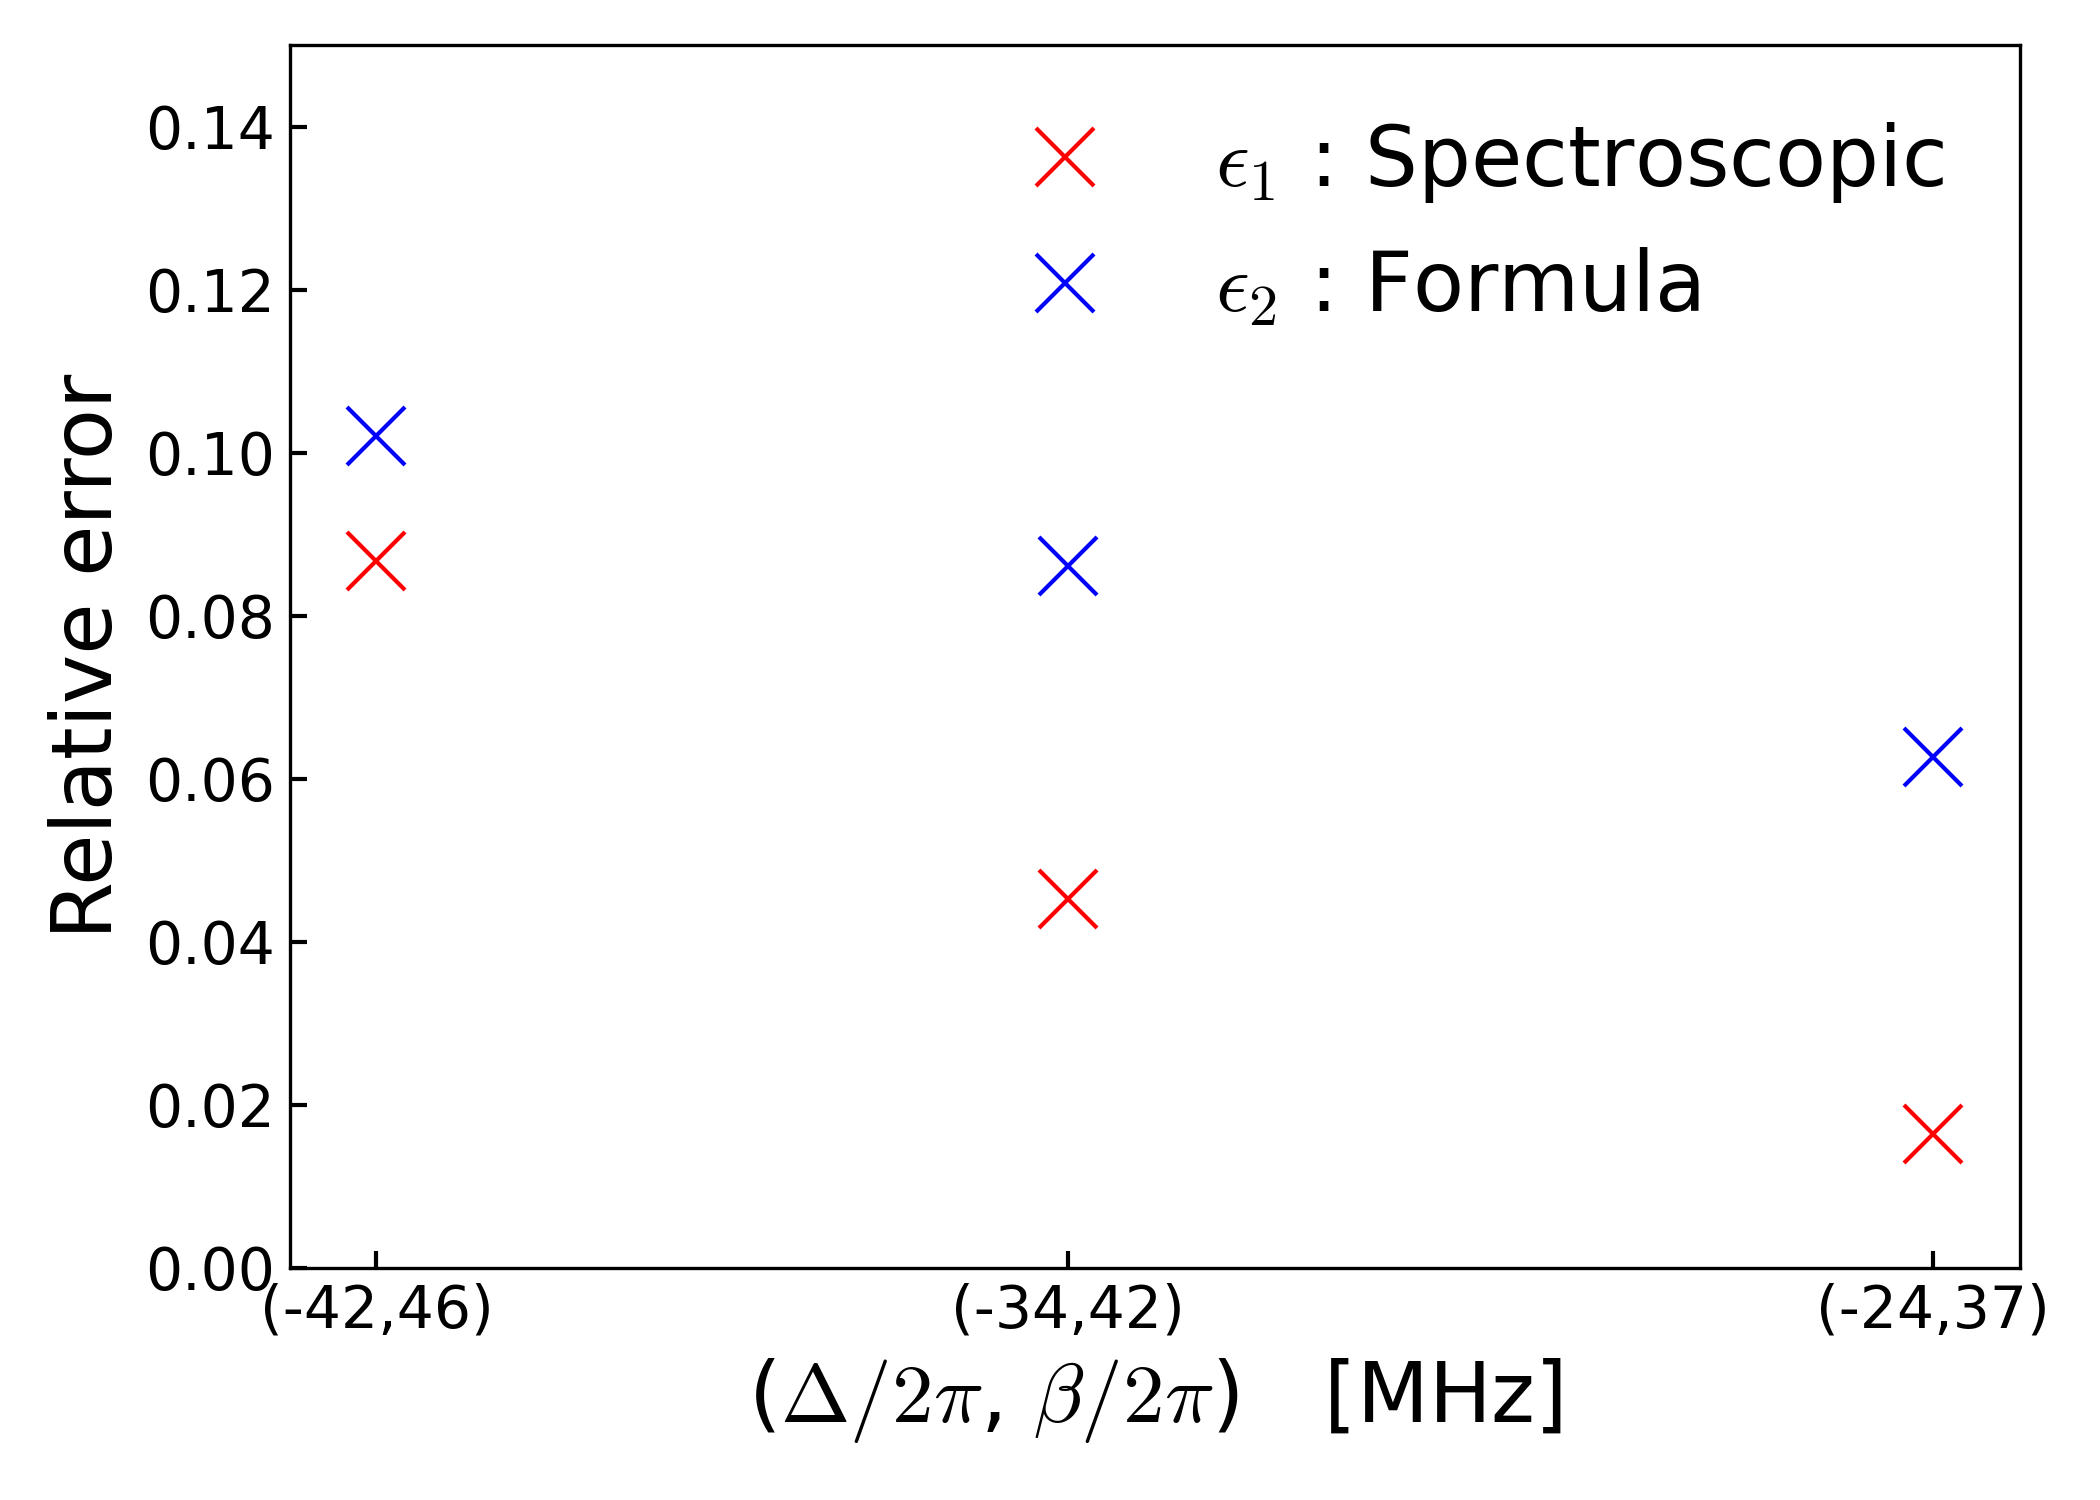
\includegraphics[width=9.1cm]{fig/alpha_estimete_meannumber2.png} \\
\caption{
Plot of 
the relative error $||\alpha_{\rm{est}}|^2-|\alpha|^2|/|\alpha|^2$ 
against the detuning of the KPO
 where $|\alpha|^2$ ($|\alpha_{\rm{est}}|^2$) is the true (estimated) value of the photon number.
We set $\beta$ to satisfy a condition of $(2\beta + \Delta)/2\pi = 50$ MHz.
Also, we set the parameters as $\chi/2\pi=18.0$ MHz, $g/2\pi=5.0$ MHz, $\lambda_{\rm{p}}/2\pi=0.5$ MHz, $\gamma_1/2\pi=\gamma_2/2\pi=0.8$ MHz, and $\omega_g=\omega_{\rm{p}}/2$.
}
\label{fig:spec_error2}
\end{figure}

\begin{figure}%[h]
\centering
		%\includegraphics[width=9.1cm]{fig/sigmaz_td_Detu_-34_Keer_18_pump_42_dec_0.8_L_2.pdf} \\
\caption{
(a) The time-integrated spectra $I$ against the detuning $\Delta_{\rm{q}}/2\pi$ with the Rabi frequency $\lambda_{\rm{p}}/2\pi=2$  MHz.
We use the same parameters as those in Fig.~\ref{fig:spect1} (a) except the Rabi frequency. 
We observe not only the main two dips but also small dips
at $\Delta _{\rm{q}}^{(3)}/2\pi=-8.40$ MHz and $\Delta _{\rm{q}}^{(4)}/2\pi=-8.65$ MHz. }

\label{fig:spec2}
\end{figure}

Also, to further quantify the performance of our method,
we calculate the relative error of our methods with other parameters, and compare the error with that of the conventional method.
When the detuning is too large for the KPO to bifurcate, the ground state of the KPO is not the superposition of the coherent states anymore. Thus, when we plot Figs.~\ref{fig:spec_error1} and \ref{fig:spec_error2}, we choose a range of detuning for the KPO to bifurcate in these numerical simulations.

% \footnote{
% When the detuning is too large for the KPO to bifurcate, the ground state of the KPO is not the superposition of the coherent states anymore. Thus, when we plot Figs.~\ref{fig:spec_error1} and \ref{fig:spec_error2}, we choose a range of detuning for the KPO to bifurcate in these numerical simulations.}.
In Fig.~\ref{fig:spec_error1}, we plot the relative error against the detuning of the KPO $\Delta$.
In Fig.~\ref{fig:spec_error2}, we plot the relative error against 
$\Delta$ by setting $\beta$ to satisfy a condition of $(2\beta + \Delta)/2\pi = 50$ MHz.
The reason why we choose this condition is that the estimated photon number $|\alpha_{\rm{ana}}|^2$ from the analytical formula is fixed in these numerical simulations.
From Figs.~\ref{fig:spec_error1} and~\ref{fig:spec_error2}, our method provides a more accurate estimate of $|\alpha|^2$ than the conventional method when there is a detuning $\Delta$. 
%\YM{In Fig.~\ref{fig:spec_error1}, we find that there is an optimal detuning to minimize the relative error
%for our method.
%This shows a non-monotonic dependence of the relative error on the detuning.
%}
Fig.~\ref{fig:spec_error1} shows a non-monotonic dependence of the relative error on the detuning. Thus, we find that there is an optimal detuning to minimize the relative error
for our method.
It is worth mentioning that, in the original proposal of QA with KPO \cite{goto2016bifurcation}, KPO has a finite detuning during QA. Therefore, our scheme is useful for such circumstances.


Furthermore, we investigate how a stronger Rabi frequency affects spectroscopic measurements.
We perform numerical simulations with a Rabi frequency
of
$\lambda /2\pi = 2$ MHz.
It is worth mentioning that
we observe not only the prominent two dips but also small dips
at $\Delta _{\rm{q}}^{(3)}/2\pi=-8.40$ MHz and $\Delta _{\rm{q}}^{(4)}/2\pi=8.65$ MHz, in Fig.~\ref{fig:spec2}.
We expect that these additional dips come from the violation of the rotating wave approximation, which  will be discussed in Appendix~\ref{purtabation}.

\subsection{photon lossによる実用上の問題について}
レフェリーによる有益なコメントに感謝する.確かに,我々の数値シミュレーションでは,光子の損失により,2つのコヒーレントな状態のインコヒーレントな混合が発生する.同様に,量子アニーリングにおける問題のハミルトニアンの基底状態が縮退している場合,光子の損失により基底状態のインコヒーレントな混合が発生します.しかし,実際の量子アニーリングでは,以下の理由により,実用上の問題は生じないはずです.量子アニーリングの主な対象である組み合わせ最適化問題では,縮退した基底状態のいずれかを得ることができれば計算は成功したとみなされる.そのため,量子アニーリング後に縮退した基底状態の古典的混合状態を得る場合,その状態を読み出すだけで,いずれかの基底状態を得ることができる.この点については,修正原稿で説明しています.

Let us remark that, although the ground state of the KPO is a superposition of two coherent states, we have a classical mixture of two coherent states in our numerical simulations
due to the photon loss.
Similary, if we perform quantum annealing with a problem Hamiltonian whose ground states are degenerate, we will obtain not the superposition of the ground states but the classical mixture between them.
Fortunately, this does not affect the performance of QA for the following reason.
When we solve combinational optimization problems with QA, the purpose is not to obtain all degenerate ground states 
but to obtain one of the ground state. So, even if the state after QA is a classical mixture of the degenerate ground states, single shot measurements of KPOs project the states into one of the ground states, and we obtain the answer. 


% \begin{figure}[h]
% \centering
% 		%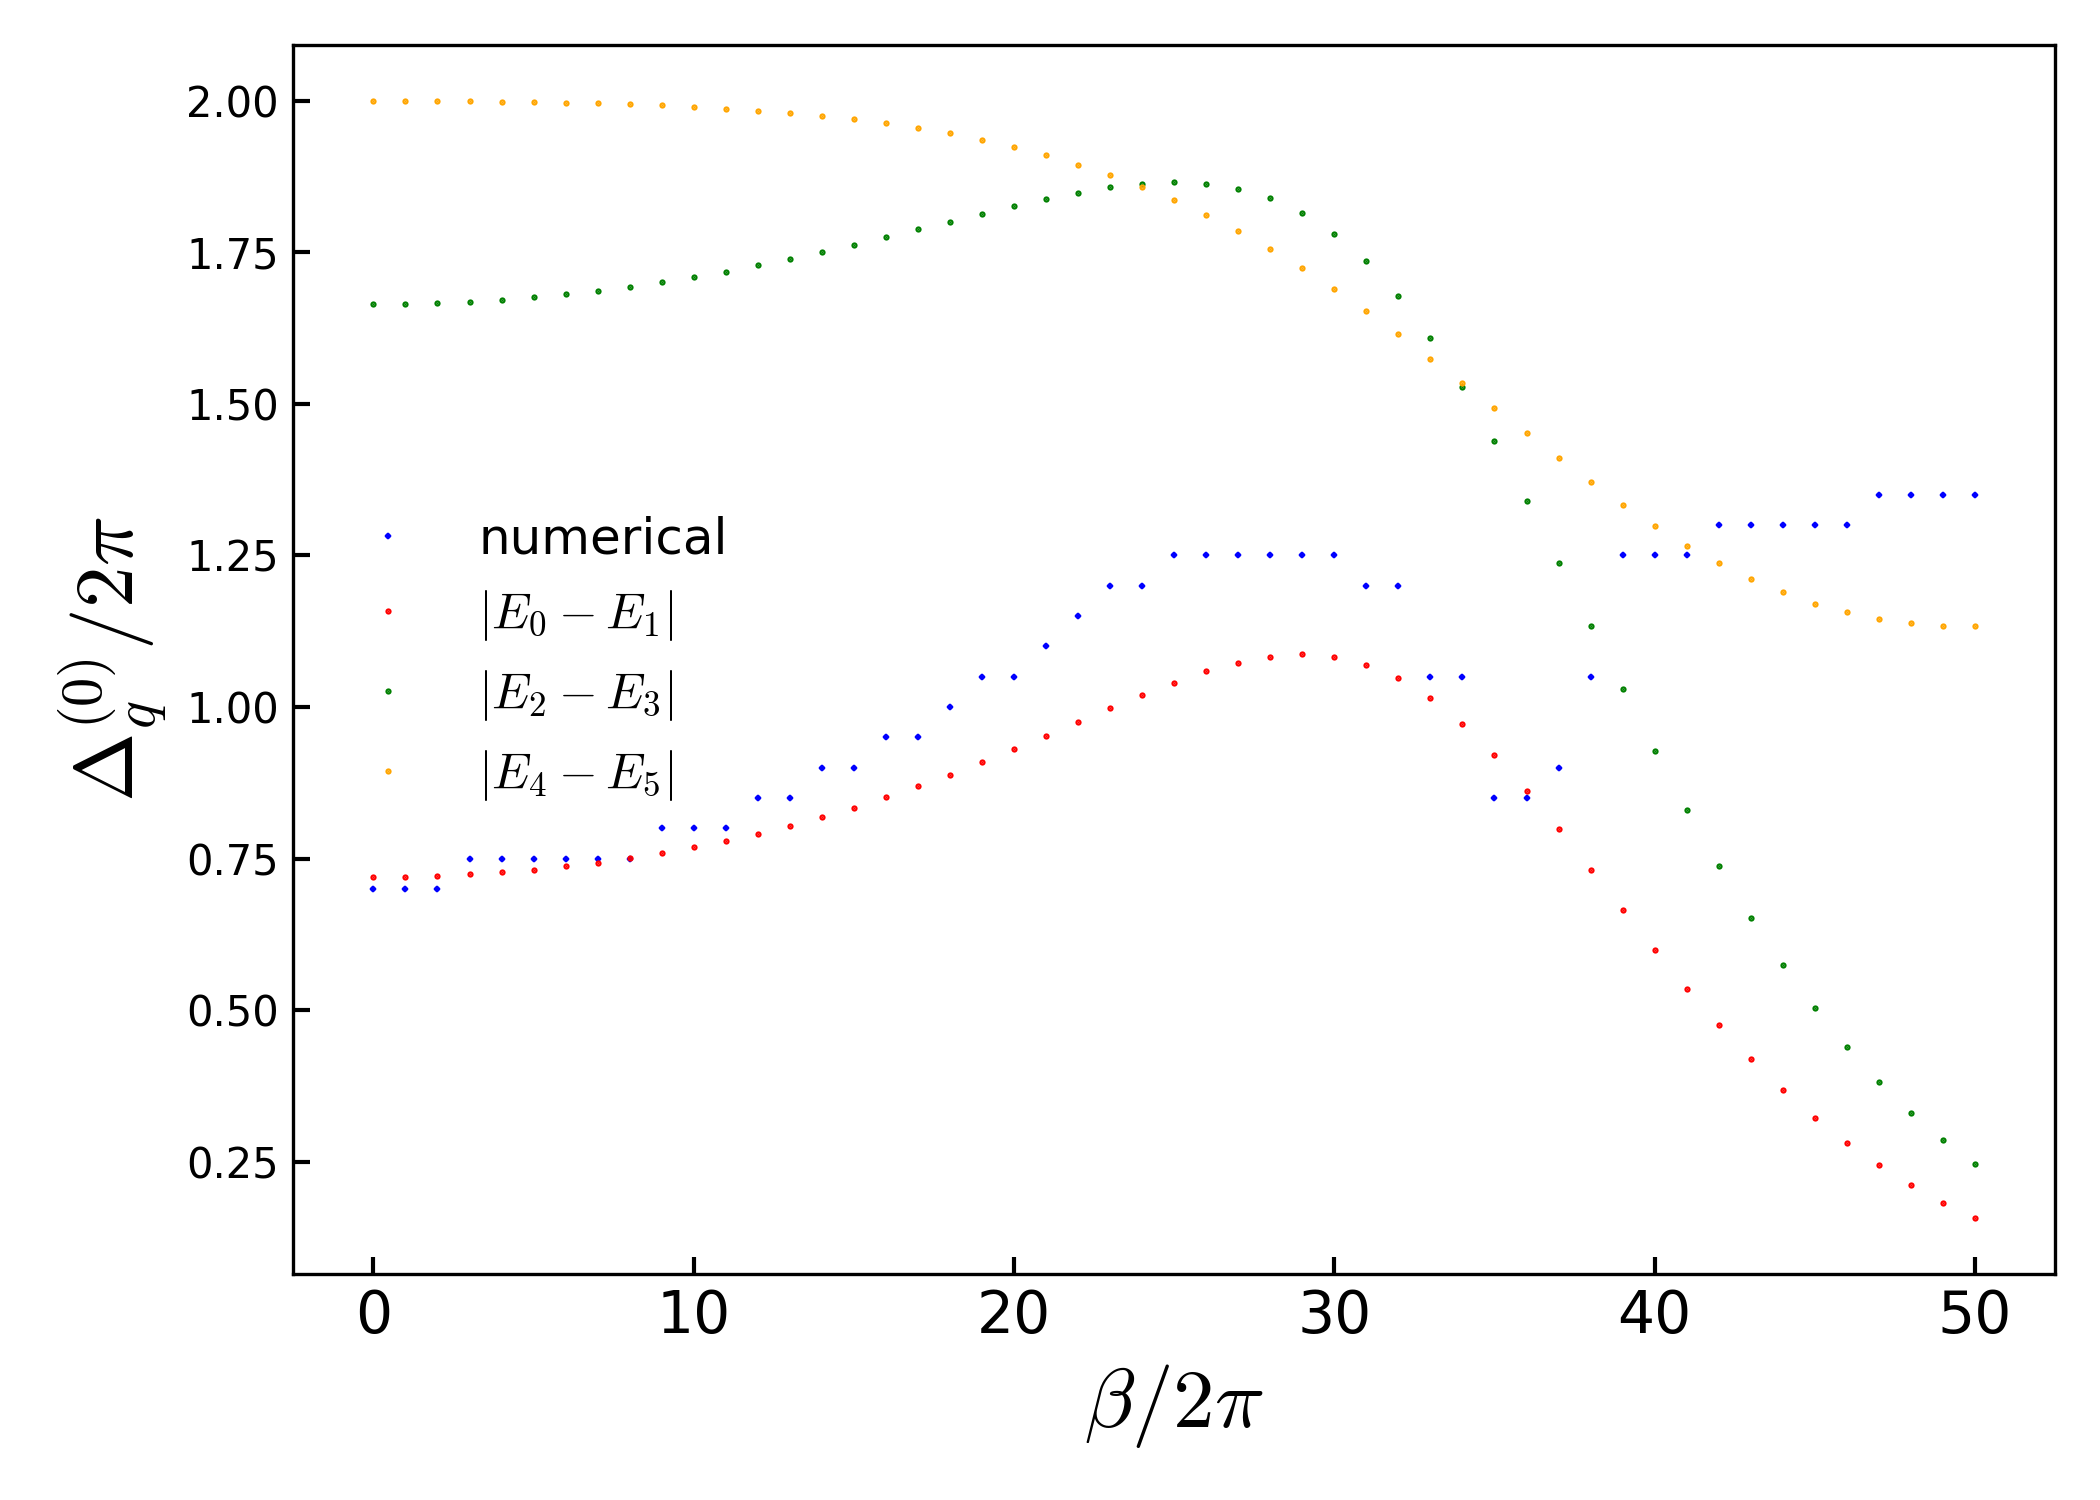
\includegraphics[width=9.1cm]{fig/spect_sigmaz_td1D_Detu_-34_Keer_18_dec_0.8_L_0.5.png} \\
% \caption{
% \KM{(a) The time-integrated spectra $I$ against $(\omega_{\rm{c}}-\omega_{\rm{p}}/2)/2\pi$ with $\lambda/2\pi = 0.5$ MHz.
% (b) Color map of the expectation values of $\hat{\sigma}_z$ againt $(\omega_{\rm{c}}-\omega_{\rm{p}}/2)/2\pi$ (x axis) for a given time (y axis) with $\lambda/2\pi = 0.5$ MHz.
% We set the parameters as $\Delta/2\pi = 100$ MHz, $\chi/2\pi = 18$ MHz, $\beta/2\pi = 20.0$ MHz, $g/2\pi = 5$ MHz.
% }The time-integrated spectra $I$ against $\Delta_{\rm{q}}/2\pi$ with $\lambda_{\rm{p}}/2\pi=0.5$  MHz. We set the parameters as $\Delta/2\pi-34.0$  MHz, $\chi/2\pi=18.0$ MHz, $\beta/2\pi=42.0$ MHz, $g/2\pi=5.0$ MHz, and $\omega_g=\omega_{\rm{p}}/2$.}
% \label{fig:pump_effect}
% \end{figure}

\section{Conclusion}
In conclusion, we propose an experimentally feasible method to estimate the number of photons of the KPO. We couple an ancillary qubit with the KPO, and spectroscopic measurements of the qubit let us know the number of photons of the KPO. Our results are essential to realize QA with KPOs for solving combinational optimization problems.




\section{議論}
松崎様

 

山本です.

少し私からもコメントさせてください.

 

今問題となっているコメントは,査読者が,

・光子数を決めるためには,Fig. 2aに相当するものを実験で測定する必要がある.

・そのためには量子ビットのσzを測定する必要がある,

・だから量子ビットの状態読出しのための共振器が必要だろう

と考えたからだと思います.

 

ですが,我々としては,Fig. 2aに相当するものは量子ビットの反射測定で測ることを意図していたので,

読出しの共振器は不要で,Fig. 1にも描いていなかったということだと思います.

 

実際のところ,読出し共振器を設けて量子ビットの状態を測定することは勿論可能ですが,

実験的には量子ビットを直接反射測定するより大分複雑になるので,

本論文で主張している簡便な方法という点が弱くなってしまいます.

 

ですので,(山口さんのメールの前に)山口さんと相談した時は,

反射測定を基本とするべき(分散読出しはオプションとしてはあり)なので,

Fig. 1には読出し共振器は描かない方が良い,と考えました.

 

そのためには,Fig. 2aに相当するものを反射測定で測れるということを,

説明できるかどうかがポイントだと思います.

例えば,材料として,

増田さんのNew J. Phys. 23 (2021) 093023の論文

(対象はKPOですが,Eq. 30, 31に反射係数と密度行列の対角成分の関係式がある)や

実験ではAstafiev et al., Science 327, 841 (2010)

(Fig. 1c 導波路に磁束量子ビットが直接結合した系の透過率が,量子ビットの励起により変化する)

が使えるのではないかと思います.

 

よろしくお願いします.

 




松崎です.
海外出張中で対応が遅れてすみません.

いろいろと考えたのですが,dispersive measument のセットアップを書きつつ,本文中(およびcaption)で,トランズモン量子ビットへプローブ光をいれて分光測定することも可能であると書くのが良い気がします.

ちなみに来週は産総研の火曜日以降にはいらっしゃいますでしょうか?
少し議論できれば幸いです.

 

お世話になっております.山口です.

お返事が遅くなり申し訳ありません.

 

Referee1からのコメントに関して,図を作成すること自体は問題ないのですが,

1点確認させてください.

今回の測定では,transmon(またはtransmon動作しているKPO)を想定していており,

それを”分光測定”するという簡便な方法で光子数がわかる,ということがミソであったと思います.

この分光測定はdispersive readout を行うのではなく,直接transmonにプローブを入れて

その反射測定をするものだと思っていたので,readout resonatorは必要ない,

と思っていたのですが,いかがでしょうか?

 

これに類する実験として,以前に私が2KPO系で測定した際には,

ポンプしていない側のKPO(今回のtransmon)を直接分光していました.

 

Dispersive readoutで同様の測定をすることも不可能ではないとは思うのですが,

簡便性という観点からも,直接の分光をする,という主張のほうがシンプルに思います.

 

以上,ご検討いただけますと幸いです.

どうぞよろしくお願いいたします.





山本様へ

いつもお世話になっております松崎です.
「
Fig. 1で

Coherent driveと書かれたポートが

それだと思います.

」

なるほど.了解いたしました.
丁寧な返信をありがとうございます.大変勉強になりました.

松崎 雄一郎


差出人: YAMAMOTO TSUYOSHI(山本 剛)
送信: 2022 年 12 月 12 日 (月曜日) 8:57
宛先: 松崎雄一郎
Cc: 松本佳大; 山口愛子
件名: RE: Our initial decision on your article: JJAP-S1102957

松崎様

 

ちなみに,我々のスキームで反射測定を行う場合,トランズモン量子ビットにtransmission lineを結合させる必要があると思いますが,その理解であっておりますでしょうか?
 

Fig. 1で

Coherent driveと書かれたポートが

それだと思います.

 

もしそうだとすると,トランズモン量子ビットにtransmission lineが結合した図が必要かと思いました.
 

上記の通り,現在の図はすでにそうなっていると私は理解しています.

 

よろしくお願いします.

山本剛

From: 松崎雄一郎 <matsuzaki.yuichiro@aist.go.jp>
Sent: Monday, December 12, 2022 8:46 AM
To: YAMAMOTO TSUYOSHI(山本 剛) <tsuyoshi.yamamoto@nec.com>
Cc: 松本佳大 <matsumoto-kei@aist.go.jp>; 山口愛子 <aiko-uchiyama@aist.go.jp>
Subject: Re: Our initial decision on your article: JJAP-S1102957

 

山本様へ

 

松崎です.返信ありがとうございます.

なるほど.反射測定でも,JPAをつかうことでsingle shot readoutが可能なのですね.

よくわかりました.

 

ちなみに,我々のスキームで反射測定を行う場合,トランズモン量子ビットにtransmission lineを結合させる必要があると思いますが,その理解であっておりますでしょうか?

 

もしそうだとすると,トランズモン量子ビットにtransmission lineが結合した図が必要かと思いました.

 

松崎雄一郎

 

 

差出人: YAMAMOTO TSUYOSHI(山本 剛)
送信: 2022 年 12 月 11 日 (日曜日) 22:31
宛先: 松崎雄一郎
Cc: 松本佳大; 山口愛子
件名: RE: Our initial decision on your article: JJAP-S1102957

 

松崎様

 

ご返信ありがとうございました.

 

反射測定もsingle-shot readoutは可能です.

 

1~10程度の平均光子数のプローブ信号強度かつ~20 dBのゲインのJPAを用いた場合,

dispersive readout,反射測定共に~100 nsが標準的な読出し時間と思います.

 

よろしくお願いします.

山本剛

From: 松崎雄一郎 <matsuzaki.yuichiro@aist.go.jp>
Sent: Sunday, December 11, 2022 8:06 PM
To: YAMAMOTO TSUYOSHI(山本 剛) <tsuyoshi.yamamoto@nec.com>
Cc: 松本佳大 <matsumoto-kei@aist.go.jp>; 山口愛子 <aiko-uchiyama@aist.go.jp>
Subject: Re: Our initial decision on your article: JJAP-S1102957

 

山本様へ

返信ありがとうございます.

 

では両方について言及して,共振器は書かない方針で行きたいと思います.

 

「

ちなみに分散読出しのほうが,反射測定よりも早く読めるとお考えの理由は何でしょうか?

スピードを決めているのは,読出し共振器や量子ビットと伝送線路の結合強度と,

読出しのプローブ信号強度と思いますが,どちらも大きな差はないように思っています.

」

 

ここは私の勘違いがあるのかもしれません.

お手数をおかけしますが,以下の私の理解が正しいか,お教え頂ければ幸いです.

 

共振器を用いてdispersive readoutができる場合は,single shot readoutが可能です.

そのため,数十ns程度で,qubitのアップかダウンかを判定できます.

 

反射測定の場合は,single shot readoutができないので繰り返し計測する必要があります.

数十nsで読む出すことは,かなり難しいと思います.

 

いかがでしょうか?

私が何か勘違いしているかもしれません.その場合は申し訳ございません.

 

松崎 雄一郎

 

 

差出人: YAMAMOTO TSUYOSHI(山本 剛)
送信: 2022 年 12 月 11 日 (日曜日) 10:41
宛先: 松崎雄一郎
Cc: 松本佳大; 山口愛子
件名: RE: Our initial decision on your article: JJAP-S1102957

 

松崎様

 

ご返信ありがとうございました.

 

両方について言及するのは良いと思います.

(私はやはり図に共振器は描かなくてよいと思います)

 

ちなみに分散読出しのほうが,反射測定よりも早く読めるとお考えの理由は何でしょうか?

スピードを決めているのは,読出し共振器や量子ビットと伝送線路の結合強度と,

読出しのプローブ信号強度と思いますが,どちらも大きな差はないように思っています.

 

よろしくお願いします.

山本剛

From: 松崎雄一郎 <matsuzaki.yuichiro@aist.go.jp>
Sent: Sunday, December 11, 2022 9:13 AM
To: YAMAMOTO TSUYOSHI(山本 剛) <tsuyoshi.yamamoto@nec.com>; 山口愛子 <aiko-uchiyama@aist.go.jp>
Cc: 松本佳大 <matsumoto-kei@aist.go.jp>
Subject: Re: Our initial decision on your article: JJAP-S1102957

 

山本様

 

いつもお世話になっております松崎です.

コメントありがとうございます.

 

「

ですので,(山口さんのメールの前に)山口さんと相談した時は,

反射測定を基本とするべき(分散読出しはオプションとしてはあり)なので,

Fig. 1には読出し共振器は描かない方が良い,と考えました.

」

 

たしかにその方針でも良いかもしれません.

 

ただ私として懸念していることを以下にあげます.

 

KPOで複雑な問題をQAで解いたときに,QAを終えた直後と,QAを終えてから(発振を続けていても)時間がたってからでは,KPOの光子数が変わる可能性があるという点です.

もちろん,T1の影響で|α>が|-α>になるだけであれば,平均光子数自体は変化しない気もします.

ただ,KPOの振る舞いは複雑なので,光子数が変わる可能性も否定はできないと思います.

 

 

反射測定で我々のプロトコルを実行する場合,KPOの光子数を読みだすのに時間がかかってしまうと思います.

dispersive測定で実行すれば,KPOの光子数を高速で読めると思います.

 

そのため,QAで終えた直後に,dispersive測定で高速にKPOの光子数を読み取れば,上のようなKPOの光子数が変わるという問題が起きないと思います.

 

ただ,この点はあくまでも懸念点程度で,実際に本当に問題になるかは自信がありません.

 

そのため両方の場合を書くのが無難かと考えております.

 

両方というのは

・高速でKPOの光子数を知りたい場合→dispersive測定

・時間をかけても良い場合→プローブによる反射測定

を説明するということです.(上の懸念点は,ちょっと自信がないので,具体的には書かないつもりです.あくまでも状況に応じて使い分けられるよね,と書く程度です)

 

その場合に,図に読み出しのためのresonatorを書くかどうかは悩ましいですが,書かないのもありかと思います.(その場合でも本文中にはdispersive測定の場合も書く予定です)

 


いかがでしょうか?
